% =============== No Touchy =================== %
\documentclass[11pt, conference, onecolumn]{IEEEtran}

\usepackage{cite}
\usepackage{amsmath,amssymb,amsfonts}
\usepackage{algorithmic}
\usepackage{graphicx}
\usepackage{textcomp}
\usepackage{xcolor}
\usepackage{caption}
\usepackage{subcaption}

\def\BibTeX{{\rm B\kern-.05em{\sc i\kern-.025em b}\kern-.08em
    T\kern-.1667em\lower.7ex\hbox{E}\kern-.125emX}}
\begin{document}

\title{A Portable Tensor Processing Unit\\
}

\author{\IEEEauthorblockN{Wesly Tonks}
\IEEEauthorblockA{\textit{UC Davis}\\
Davis, United States \\
watonks@ucdavis.edu}
\and
\IEEEauthorblockN{Cameron Shinn}
\IEEEauthorblockA{\textit{UC Davis}\\
Davis, United States \\
ctshinn@ucdavis.edu}
\and
\IEEEauthorblockN{Alan Qin}
\IEEEauthorblockA{\textit{UC Davis}\\
Davis, United States \\
aqin@ucdavis.edu}
\and
\IEEEauthorblockN{Skye Develasco}
\IEEEauthorblockA{\textit{UC Davis}\\
Davis, United States \\
sdevelasco@ucdavis.edu}
}

\maketitle

% ============ End No Touchy ==================%

\begin{abstract}
    Trends in computing have led to a proliferation of Neural Network applications.
    Unfortunately, todays general purpose processors are not well suited for the class of
    computations these applications require, creating demand for a new class of processors
    - Tensor Processing Units (TPU). These hardware accelerators are designed with Neural
    Networks in mind, and allow host CPUs to offload computationally expensive
    tensor operations to them. We implement our own, low-power, scalable TPU intended for
    embedded and mobile applications, and evaluate its performance using a simulated
    fully connected Neural Network layer.
\end{abstract}

\begin{IEEEkeywords}
Neural Networks, Machine Learning, TPU, Hardware Acceleration
\end{IEEEkeywords}

\section{Introduction}
    % Big Picture
    % Motivation
    % Problem Definition
    % Objective
    With the diminishing of Moore's Law and the exponential increase in data, computing
    needs are out-pacing computing capabilities in general purpose processors in both
    client and server applications. Today's solution is the design of specialized hardware
    co-processors, which specialize in one or a few tasks. These hardware accelerators
    perform complex computations much faster (on the order of 10 - 100 times faster), and
    with much lower power consumption. With the increasing expense of power in all parts
    of the computing spectrum, it is no wonder that hardware accelerators are becoming
    ubiquitous.

    With the creation of data accelerating at an exponential rate, algorithms to
    extrapolate useful information - namely Neural Networks, have become
    common, and are found in embedded, mobile, and data center applications. These
    algorithms rely heavily on matrix multiplication and convolution, both of which place
    heavy load on today's general purpose processors, creating the need for a Tensor
    Processing Unit (TPU), first commercialized by Google for data center use.

    Note that Neural Networks has two phases: training and predicting. Both phases are
    computationally expensive, and the topic of cutting edge research. Here, we focus
    on predicting, as much of the neural networks life will be spent making predications,
    rather than training.

    Current TPU's aim to implement the aforementioned matrix multiplication and
    convolution, along with common activation functions used in todays Neural Networks.
    This is typically done via a highly pipelined data path known as a systolic array,
    which can complete an $N x N$ matrix multiplication in just $2N$ cycles. As with most
    hardware accelerators, TPU's must communicate large amounts of data between itself and
    the host, introducing undesired overhead. TPU's also have large on chip memory
    bandwidth, as the systolic array requires large input and output bandwidth for sustained
    computation.

    The TPU was first introduced by Google in 2013, who was presented with a massive
    amount of compute as their customers began using speech-to-text more often. Over the
    course of 15 months, Google designed and fabricated their fist generation TPU, and
    was able to realize fantastic performance improvements in neural network inference,
    and now uses their TPU as an add in card in their own data centers.

    We present a scaled down, low-power TPU implementation providing performance gains for
    embedded and mobile neural network applications. We aim to increase performance of
    fully connected layers in an application running on an ARM A9 processor. The TPU is
    memory mapped, and communication between the two devices is done via an Avalon bus on
    an Altera DE-1 development kit. The TPU implements a fully pipelined 16 x 16 systolic
    array at a max clock speed of 115 MHz, yielding a noticeable speedup in
    fully connected neural network layers, when compared to the ARM A9 only.

    This implementation allows useful Neural Network applications such as image processing,
    object detection, speech-to-text, and more to be run in power and performance limited
    devices such as smart phones and embedded systems. The design is also scalable,
    allowing for a range of hardware configurations per application.
\section{Background}

\subsection{Neural Networks}
    % General description of neural networks here.
    With the advent of big data applications becoming increasingly common, machine learning
    has proved to be the future of complex algorithms. Deep neural networks, a subspace of
    machine learning, are an attempt to reverse engineer the human brain and make computers
    learn and behave like humans. Deep neural networks need to first undergo “training”
    repeatedly with vast amounts of sample data, and self adjusted “synapses”
    (i.e. learning) based on expected results. If given a complete dataset, it is typical
    to use 20\% of the data to train the network, and 80\% to test it. Once a neural
    network has been fully trained, it can then be applied and performs  “inference” on
    whatever it is given. This implies that a domain specific architecture should take
    advantage that weights will always remain the same, as will be shown later.

    Neural networks are essentially just a series of simple functions applied independently
    to each part of an input. This allows matrices to be used, as matrix operations apply
    the same operation to each piece of the inputs. The downside is that common matrix
    operations such as multiplication and convolution are exceedingly complex, meaning
    general purpose processors (and even GPUs) have low roofline performance for
    neural network inference.

\subsection{Tensor Processing Units}
    % Present the need for Tensor Processing Units
    % Talk about Google's implementation
    % Talk about need for portable, low power TPUs
    Since Moore's law and Denard scaling are coming to an end, industry is adopting
    domain specific architectures which promise extremely high price-performance-power for
    a given set of problems. Google's own TPU is a great example, yielding much greater
    throughput and performance per watt than top GPU's and CPU's in Neural Network
    Inference. The success of Google's first generation TPU led to faster and more power
    efficient generations which are now used throughout Google's data centers.

    Google's TPU first came about when researchers at Google proposed a problem - what
    would happen if every Google user used speech-to-text services for just three minutes
    a day? They found that the amount of compute needed would far exceed the capabilities
    of their CPU and GPU driven data centers, and 15 months later produced a fully
    functional TPU.

    Google's TPU consists of a large $256 x 256$ Systolic array which performs fast matrix
    multiplication. THe systolic array is a 2-dimensional array of processing elements
    (PE's) which are relatively simple execution units. At minimum, they contain a
    registers, a multiply accumulate module, and some control logic. Each PE receives a
    sum, weight, and input matrix element as inputs, and multiplies the input matrix
    element by the weight, then adds that to the sum. The sum is then passed downwards
    to the next PE, while the input matrix element is passed right to another PE. After
    a short transient, Google's Systolic array performs $256^2$ multiply-accumulates per
    clock cycle, allowing massive throughput.

    While the large systolic array is capable of massive amounts of compute, it may only
    do so if memories can feed it. Because a set of weights for a given network is usually
    too large to store in on-chip caches, Google uses a DDR3 interface to hold weights,
    put hides memory latency by using Weight FIFO's to prep a set of weights while a
    multiply is taking place. A similar technique is used for the input matrix, which must
    through the 'data set-up' block, as shown below.

    \newpage

    \begin{figure}[htbp]
        \centering
        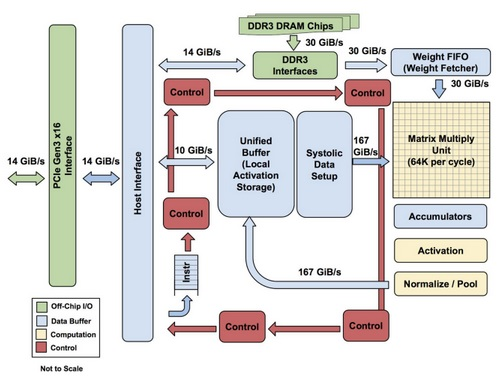
\includegraphics[width=9cm]{../figures/googleArchitecture.jpg}
        \caption{High level view of system Architecture}
    \end{figure}

    Google’s original TPU is far more efficient than CPUs and GPUs with 30X to
    80X the energy efficiency (TOPS/Watt), not to mention it’s currently in its third
    generation. The performance of the TPU in a data center environment is unparalleled
    and offers an excellent solution to deep neural network inference in the cloud computing
    space.


\section{Design and Implementation}

    \subsection{System Architecture}
        % Inspiration from Google
        % Include system Architecture figure
        We give credit to Google's TPU as inspiration for our own architecture. Given the
        level of design we are at, resources describing Google's TPU proved very helpful
        in implementing our own.

        A basic overview of our architecture is shown below. Commands and data flow in
        from the host interface, an Avalon AXI bus. These commands are decoded into one of
        the following functions:

        \begin{center}
        \begin{itemize}

            \item{\textit{Write Weight Memory} - Data on the bus is written into a
            specified location in Weight Memory space}

            \item{\textit{Write Input Memory} - Data on the bus is written into a
            specified location in Input Memory space}

            \item{\textit{Fill Weight FIFO's} - A set of weights is read from weight
            memory into the weight FIFO's}

            \item{\textit{Drain Weight FIFO's} - The set of weights currently held in
            the weight FIFOs is loaded into the systolic array}

            \item{\textit{Matrix Multiply} - A set of inputs is piped into the systolic
            array and multiplied with the set of weights currently held in the array.}

            \item{\textit{Read Output Memory} - A specified word from memory is read to
            the host.}
        \end{itemize}
        \end{center}

        \begin{figure}[htbp]
            \centering
            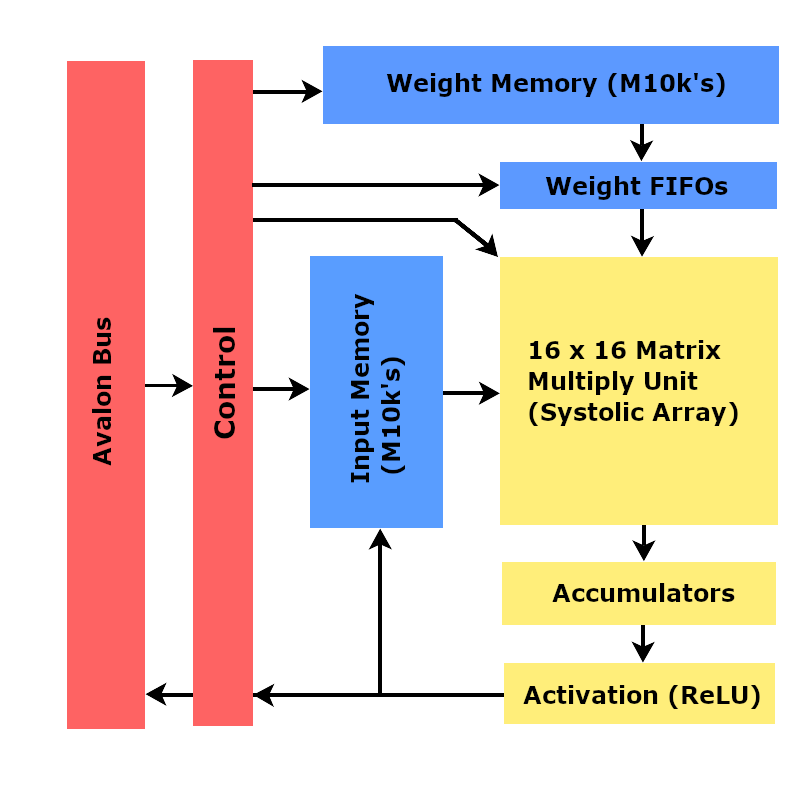
\includegraphics[width=9cm]{../figures/sysArchitecture.png}
            \caption{High level view of system Architecture}
        \end{figure}

    \subsection{Systolic Array}
        % Overview of systolic array
        % Include overview of PE
        % How memory is able to feed the Systolic Array
        Our TPU features a weight stationary systolic array, meaning a set of weights may
        be loaded in once but used for many operations. The array is fully pipelined,
        performing a 16 x 16 matrix multiply in just 32 cycles. It is composed of many
        processing elements (PEs), which contain a small amount of memory and control
        logic, and a single multiply accumulate data path.

        A complete Matrix Multiply starts at the top left corner of the Systolic array,
        and is piped diagonally downward. In the first cycle of a multiply, input memory
        supplies data for only the top left PE. After one cycle, the first PE
        activates its neighbors below and to the right, creating the diagonally downward
        piping.

        Each PE holds one element of the input matrix in any given cycle, and passes that
        element to its right neighbor every cycle. The multiply accumulate result is
        passed downward to the neighbor below every cycle. Each PE then multiplies its
        input element with the weight element stored in it, then adds that value to the
        sum being supplied from its above neighbor. Note that memory interfaces only exist
        at the edges of the systolic array.

        Multiplication results appear at the bottom of the systolic array 16 cycles after
        a multiplication is started, and continue flowing out for 16 cycles. The flow of
        data is illustrated below, showing a scaled down version of our systolic array.

    \subsection{Software}
        % Original Goal
        % Drawbacks of hardware
        % Final benchmark
        The original goal of our application was to implement a Convolutional Neural
        Network whose input was a chest X-Ray of a human patient, and whose output was a
        set of medical diagnoses ranging from pneumonia to hernia. The neural network
        was designed using a header only library known as TinyDNN, which boasts small
        code size for limited performance processors such as our ARM A9.

        % Cameron Can you expand on the network architecture here

        Out TPU would be used alongside TinyDNN, allowing the A9 processor to offload and
        optimize matrix operations, including Multiplication and Convolution.
\section{Results}
    % Discuss Quality of implementation
    % Observed Speedup
    \subsection{Final Implementation}
        The final implementation of our TPU is quite simple. It has three memory modules,
        one each for input, weight, and output matrices, and can perform a single 16 x 16
        multiply at a time. Surprisingly, this simple implementation was enough to
        see noticeable performance gains when compared to the typical $O(n^3)$ matrix
        multiply algorithm, even with compiler optimizations!

\section{Future Work}
    % There is plenty of room for improvement of the TPU we have implemented...
    There remains a plethora of future work to be done. Our resulting implementation is
    extremely bare bones, as we had issues controlling more complex features including
    accumulation (for larger matrix operations) and ReLU activation.

    Given the amount of FPGA fabric unused by our design, it would also be beneficial to
    create a separate convolution data path, allowing the TPU to be useful for
    convolutional neural networks.

    An idea that came to us late in development was to include a small set of registers
    within each PE, rather than just a single one bit register. This would enable dynamic
    switching of weight sets in a single cycle, reducing the overhead of loading weights
    into the array.

\section*{References}

\begin{thebibliography}{00}
\bibitem{b1} G. Eason, B. Noble, and I. N. Sneddon, ``On certain integrals of Lipschitz-Hankel type involving products of Bessel functions,'' Phil. Trans. Roy. Soc. London, vol. A247, pp. 529--551, April 1955.
\bibitem{b2} J. Clerk Maxwell, A Treatise on Electricity and Magnetism, 3rd ed., vol. 2. Oxford: Clarendon, 1892, pp.68--73.
\bibitem{b3} I. S. Jacobs and C. P. Bean, ``Fine particles, thin films and exchange anisotropy,'' in Magnetism, vol. III, G. T. Rado and H. Suhl, Eds. New York: Academic, 1963, pp. 271--350.
\bibitem{b4} K. Elissa, ``Title of paper if known,'' unpublished.
\bibitem{b5} R. Nicole, ``Title of paper with only first word capitalized,'' J. Name Stand. Abbrev., in press.
\bibitem{b6} Y. Yorozu, M. Hirano, K. Oka, and Y. Tagawa, ``Electron spectroscopy studies on magneto-optical media and plastic substrate interface,'' IEEE Transl. J. Magn. Japan, vol. 2, pp. 740--741, August 1987 [Digests 9th Annual Conf. Magnetics Japan, p. 301, 1982].
\bibitem{b7} M. Young, The Technical Writer's Handbook. Mill Valley, CA: University Science, 1989.
\end{thebibliography}
\end{document}
